\documentclass[xcolor=table]{beamer}
\usepackage{etex}
\usepackage[absolute,overlay]{textpos}
\usepackage{lmodern}
\usepackage[T1]{fontenc}
\usepackage[utf8]{inputenc}
\usepackage[magyar]{babel}
\usepackage{standalone}
\usepackage{adjustbox}
\usepackage{varwidth}
\usepackage{tikz}

\usetikzlibrary{shapes, positioning, mindmap, arrows.meta, backgrounds, fit}
\newcommand{\tikzmark}[1]{\tikz[overlay,remember picture] \node (#1) {};}

\setbeamercolor{framesource}{fg=gray}
\setbeamerfont{framesource}{size=\tiny}

% straight from http://tex.stackexchange.com/a/55849/8785
  \tikzset{
    invisible/.style={opacity=0},
    visible on/.style={alt={#1{}{invisible}}},
    alt/.code args={<#1>#2#3}{%
      \alt<#1>{\pgfkeysalso{#2}}{\pgfkeysalso{#3}} % \pgfkeysalso doesn't change the path
    },
  }
\title{A PLanG programozási nyelv kiterjesztése}
\subtitle{Önálló laboratóriumi beszámoló}
\author{Scipiades Ármin\\\bigskip Konzulens: Dr.\thinspace Feldhoffer Gergely}
\date{2015. május 27.}

\usetheme{Rochester}
\usecolortheme{beaver}
\setbeamertemplate{navigation symbols}{}

\newcommand{\source}[1]{\begin{textblock*}{4cm}(8.7cm,9cm)
    \begin{beamercolorbox}[ht=0.5cm,right]{framesource}
        \usebeamerfont{framesource}\usebeamercolor[fg]{framesource}{#1}
    \end{beamercolorbox}
\end{textblock*}}

\begin{document}

\frame{\titlepage}

\begin{frame}
	\frametitle{A PLanG programozási nyelv}
	\centering
	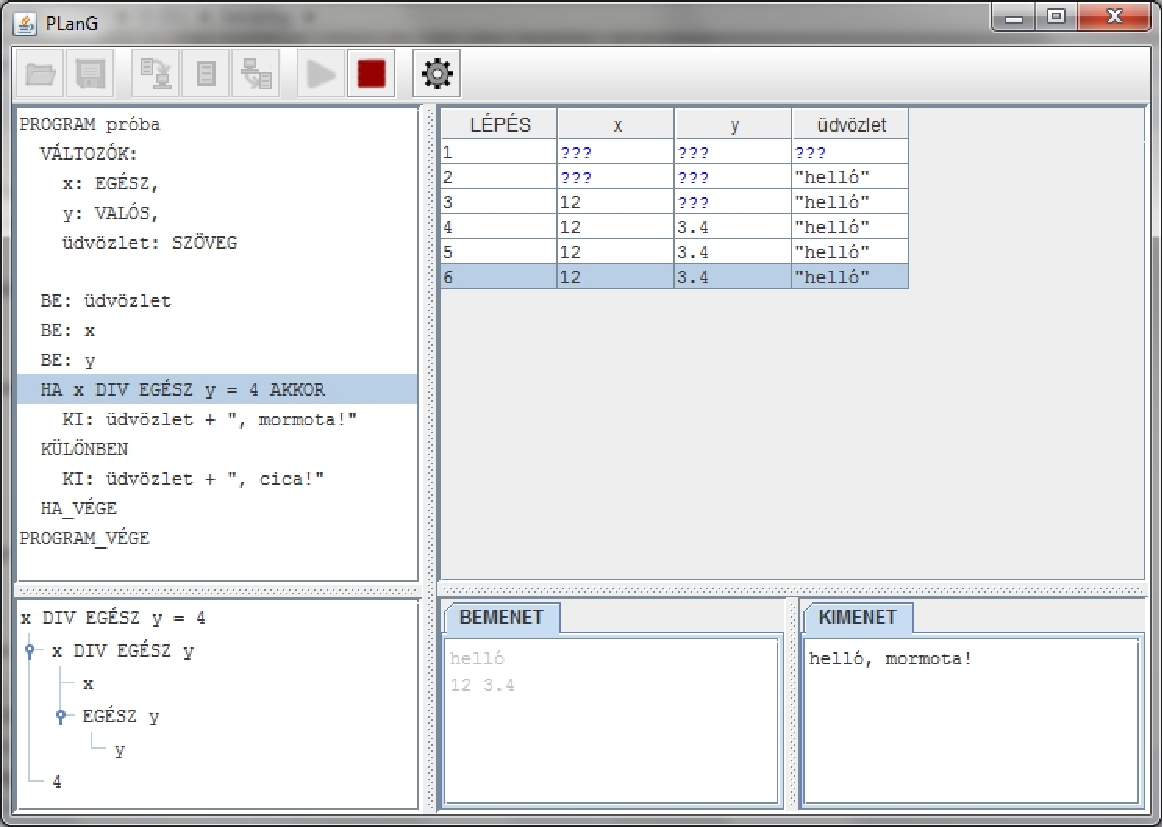
\includegraphics[width=\linewidth,height=\textheight,keepaspectratio]{images/plang.pdf}
\end{frame}

\begin{frame}
	\frametitle{A PLanG hiányosságai}
	\centering
	\begin{adjustbox}{max totalsize={\textwidth}{\textheight},center}
	
\begin{tikzpicture}
\node[text width=10cm, opacity=0.6] (language) {{\includestandalone[width=\textwidth]{images/skull_and_crossbones}}};
\end{tikzpicture}

	\end{adjustbox}
\end{frame}

\begin{frame}
	\frametitle{Objektív értékelés?}
	\centering
	
\includegraphics{images/subjective_kloran.png}
	
	\source{Michael Kloran illusztrációja}
\end{frame}

\begin{frame}
	\frametitle{A programozási nyelv felhasználói felület}	
	\centering
	\begin{adjustbox}{max totalsize={\textwidth}{\textheight},center}
	\begin{tikzpicture}[
	node distance=10cm,
	stuff/.style={draw, cloud, cloud ignores aspect, font=\Huge},
	img/.style={text width=3cm, minimum height=3cm},
	arr/.style={->, >={Latex[length=0.4cm]}},
	label/.style={above, fill=white, font=\Huge}
]

\node[stuff] (input) {Feladat};
\node[img, below= 3cm of input] (human) {{\includestandalone[width=\textwidth]{images/human_head}}};
\node[img, right of=human, text width=6cm] (language) {{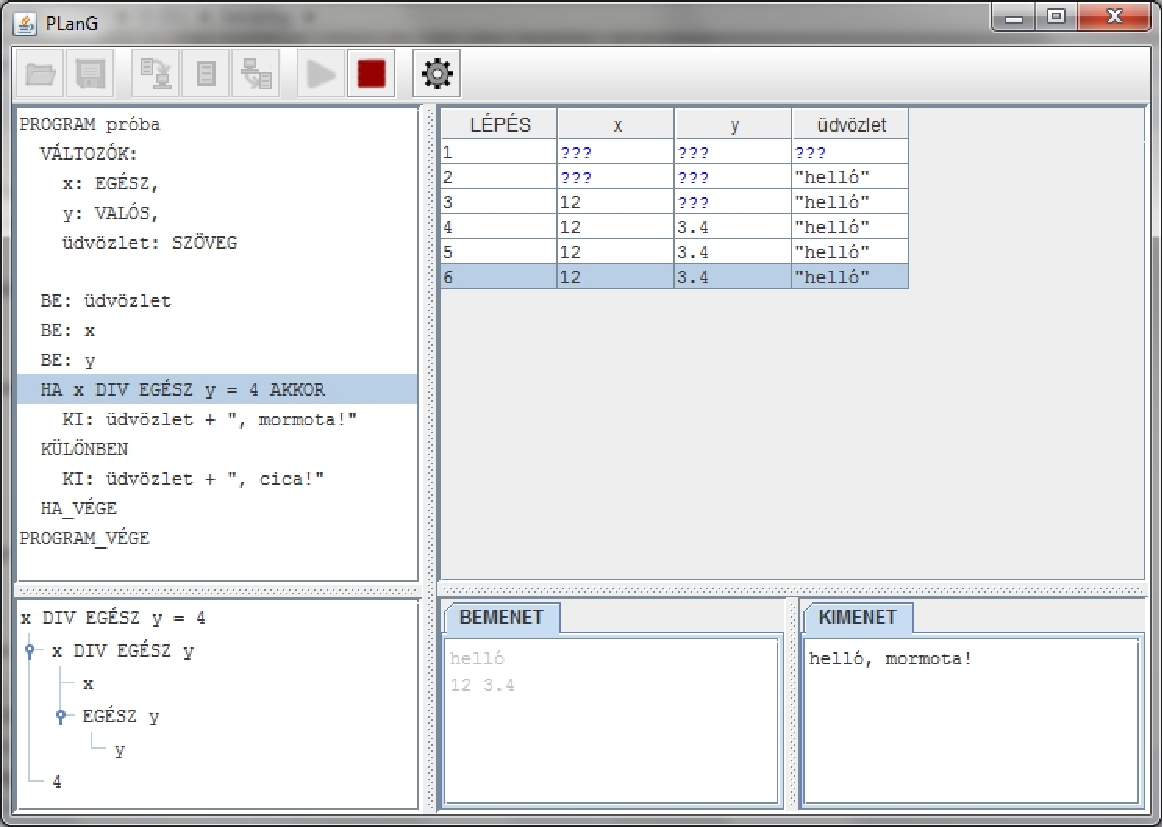
\includegraphics[width=\textwidth]{images/plang.pdf}}};
\node[img, right of=language] (computer) {{\includestandalone[width=\textwidth]{images/computer}}};
\node[stuff, above=3cm of computer] (output) {Megoldás};

\draw[arr] (input) edge (human);
\draw[arr] (human) edge node[label] {algoritmus} (language);
\draw[arr] (language) edge node[label] {program} (computer);
\draw[arr] (computer) edge (output);

\end{tikzpicture}

	\end{adjustbox}	
\end{frame}

\begin{frame}
	\frametitle{Programozási nyelvek minőségi mutatói}
	\centering
	\begin{adjustbox}{max totalsize={\textwidth}{\textheight},center}
	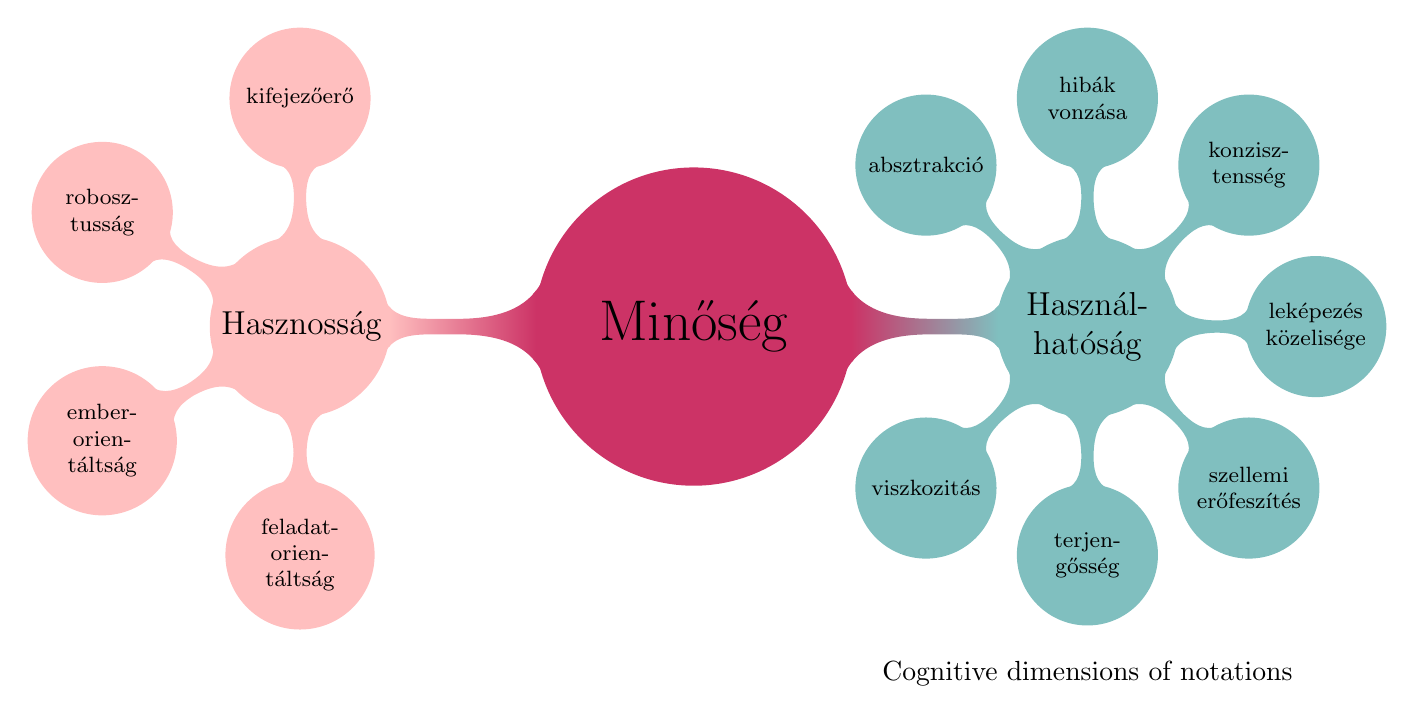
\begin{tikzpicture}
	\path[
		mindmap,
		concept color=purple!80,
		text=black
	]
		node [concept, font=\huge] {Minőség}
		[clockwise from=0, level 1 concept/.append style={sibling angle=180}]
		child[concept color=teal!50] {
			node[concept, font=\large] (usability) {Hasz\-nál\-ha\-tó\-ság}
			[clockwise from=135, level 2 concept/.append style={sibling angle=45, visible on=<3->}]
			child { node[concept] {absztrakció} }
			child { node[concept] {hibák vonzása} }
			child { node[concept] {kon\-zisz\-tens\-ség} }
			child { node[concept] {leképezés közelisége} }
			child { node[concept] {szellemi erőfeszítés} }
			child { node[concept] {ter\-jen\-gős\-ség} }
			child { node[concept] {viszkozitás} }
		}
		child[concept color=pink] {
			node[concept, font=\large] {Hasznosság}
			[counterclockwise from=90, level 2 concept/.append style={sibling angle=60, visible on=<2->}]
			child { node[concept] {ki\-fe\-je\-ző\-e\-rő} }
			child { node[concept] {ro\-bosz\-tus\-ság} }
			child { node[concept] {ember\-orien\-táltság} }
			child { node[concept] {feladat\-orien\-táltság} }
		};

		\node[below=3 of usability, visible on=<3->] {Cognitive dimensions of notations};
\end{tikzpicture}

	\end{adjustbox}
\end{frame}

\begin{frame}
	\frametitle{A PLanG minőségi mutatói}
	\centering
	\begin{tabular}{ r c c }
\bfseries kognitív dimenzió						& \bfseries PLanG	 & \bfseries ideális oktatási nyelv  \\
\rowcolor{red!30}		\bfseries absztrakció 		&nincs & alacsony \\
\rowcolor{red!30}		\bfseries hibák vonzása 	&közepes & nagyon alacsony \\
\rowcolor{green!30}		\bfseries konzisztensség 	&közepes & közepes  \\
\rowcolor{red!30}		\bfseries leképezés közelisége &közepes-alacsony & nagyon magas \\
\rowcolor{red!30}		\bfseries szellemi erőfeszítés &közepes & alacsony \\
\rowcolor{yellow!30}		\bfseries szerepkifejezés &közepes-magas	& magas \\
\rowcolor{yellow!30}		\bfseries terjengősség &alacsony-közepes	& közepes \\
\rowcolor{red!30}		\bfseries viszkozitás &közepes-magas	& alacsony
	\end{tabular}
\end{frame}


\begin{frame}
	\frametitle{Parametrizálható fordítóprogram}
	\centering
	\begin{adjustbox}{max totalsize={\textwidth}{\textheight},center}
	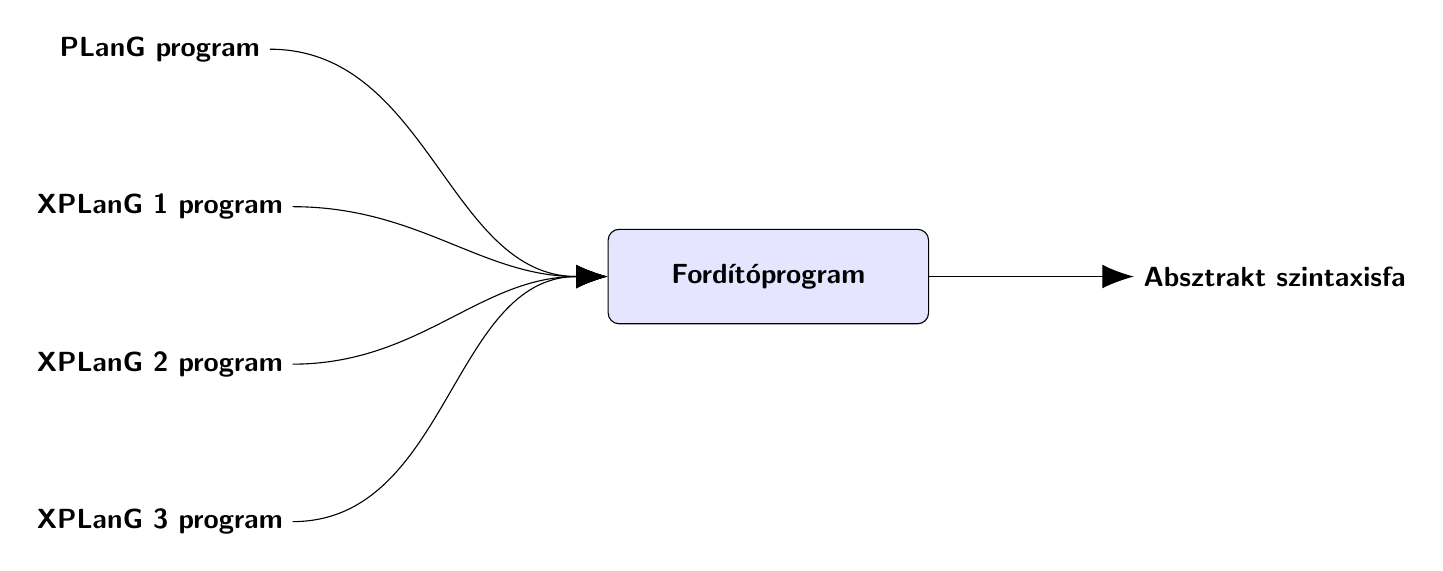
\begin{tikzpicture}[node distance=2cm,
	every node/.style={font=\bfseries\sffamily},
	clas/.style={rectangle, rounded corners, draw, fill=blue!10, inner sep=1pt, text width=4cm, text badly centered, minimum height=1.2cm},
	arr/.style={->, >={Latex[length=0.4cm]}}
	]

\node (1es) {PLanG program};
\node[below of=1es] (2es) {XPLanG 1 program};
\node[below of=2es] (3as) {XPLanG 2 program};
\node[below of=3as] (4es) {XPLanG 3 program};

\node[clas, below right=0cm and 4cm of 2es] (interpreter) {Fordítóprogram};

\node[right=2.6cm of interpreter] (out) {Absztrakt szintaxisfa};

\path[arr]
(1es) edge[out=0, in=180] (interpreter)
(2es) edge[out=0, in=180] (interpreter)
(3as) edge[out=0, in=180] (interpreter)
(4es) edge[out=0, in=180] (interpreter)
(interpreter) edge (out);


\end{tikzpicture}

	\end{adjustbox}
\end{frame}

\begin{frame}
	\frametitle{A prototípus adatfolyam diagramja}
	\centering
	\begin{adjustbox}{max totalsize={\textwidth}{\textheight},center}
	\begin{tikzpicture}[node distance=1cm,
	every node/.style={node distance=2cm, },
	clas/.style={rectangle, rounded corners, draw, fill=blue!10, inner sep=1pt, text width=2.4cm, text badly centered, minimum height=1.2cm, font=\bfseries\sffamily},
	arr/.style={->, >=latex', shorten >=1pt}
	]

\node[clas] (parser) {Parser};
\node[clas, above=of parser] (grammar) {Grammar};
\node[clas, left=of parser] (lexer) {Lexer};
\node[clas, below left=2 and 1 of parser] (context) {Context};
\node[clas, below right=2 and 1 of parser] (typechecker) {Typechecker};

\node[clas, left=of lexer] (source) {Forrásszöveg};
\node[clas, right=of parser] (interpreter) {AST Interpreter};

\path[arr, every node/.style={font=\itshape\footnotesize,
  		fill=white,inner sep=3pt}]
(source) edge node[above] {karakterek} (lexer)
(parser) edge [bend left=30] node {új állapot} (context)
(context) edge[bend left=30] node {állapot} (parser)
(grammar) edge node[above] {szabály} (parser)
(lexer) edge  node[above] {tokenek} (parser)
(parser) edge[bend right=30] node {AST-node} (typechecker)
(typechecker) edge[bend right=30] node {helyes AST-node} (parser)
(context) edge[bend right=15] node {állapot} (typechecker)
(parser) edge node[above] {AST} (interpreter);

\end{tikzpicture}

	\end{adjustbox}
\end{frame}


\begin{frame}[fragile]
	\frametitle{XPLanG}
	\centering
	\begin{adjustbox}{max totalsize={\textwidth}{\textheight},center}
	
\subsection{Követelményfeltárás}

Mint minden szoftverfolyamatnak, a nyelvtervezés első fázisa is a követelmények feltárása: a nyelv feladatterének elemzése, a felhasználói igények felmérése.
Célszerű lett volna kérdőíves felmérést végezni elsőéves diákok részvételével, komolyabban kutatni a nyelvek pedagógiai aspektusait, illetve elemezni lehetett volna az egyetem rendelkezésére álló nagyméretű korpuszt; erre erőforrások hiányában nem került sor.

Mivel létező nyelv kiterjesztéséről van szó, elemezni kellett a létező nyelvet is \aref{subsubsec:edulang}. részben ismertetett metrikák szerint.

\subsubsection{A PLanG programozási nyelv értékelése}


A PLanG első pillantásra szembetűnő jellegzetessége, hogy kulcsszavai magyar nyelvűek, ami magyar diákok számára növelheti a szerepkifejező erőt.
Mégis sok kulcsszó esetlen, furcsa megfogalmazású (\plang{MEGNYIT}, \plang{KI}, \plang{KEREK}, \plang{RND}), bár rövid (ami csökkenti a terjengősséget).
Míg az angol programozási nyelvek kulcsszavai, függvénynevei rendszerint felszólító módú igék, addig a PLanG módszeresen főneveket és mellékneveket használ, még a függvénynevekre is.
Az ilyen függvények, utasítások szerepkifejező ereje alacsony (vajon \plang{KEREK 10.5} kerekíti az értéket, vagy azt mondja meg, kerek szám-e az érték? a \plang{NAGY 'z'} azt mondja, nagybetű-e a paraméter vagy nagybetűvé alakít?).
A kulcsszavak közül a \plang{CIKLUS} nem feltétlen érthető egy olyan diáknak, aki még soha nem programozott; szerepkifejezőbb lehetett volna például az *\plang{ISMÉTELD} kulcsszó.

Az operátorok között is vannak alacsony szerepkifejezésű elemek: az \plang{@} infix operátor jelentése még gyakorlott programozóknak sem nyilvánvaló, de nem magától értetődő az sem, hogy a \plang{/=} az áthúzott egyenlőségjel helyett áll, és a \plang{DIV} és a \plang{/} osztások közül sem evidens, melyik melyik.
Hasonlóképp, bár kis programozói előképzettséggel ,,nyilvánvaló'' a \plang{:=} értékadó utasítás szemantikája, kezdőknek nem feltétlen az: anekdotikus bizonyíték szerint viszonylag gyakori hiba, hogy a diák nem tudja, melyik oldal adja, és melyik kapja az értéket.
Valóban, a \plang{:=} jó példája a \textit{memetikus kompatibilitásnak}, vagyis hogy csak azért csinálunk valamit úgy, mert mások is úgy csinálták, és nem vesszük figyelembe az eltérő igényeket\cite[6.1.5.2. rész]{McIver01}.
Szintén alacsony a tömbdeklarációk szerepkifejező ereje (\plang{EGÉSZ[5]}), ez is a memetikus kompatibilitásra törekvésből fakad.

Az I/O utasítások szerepkifejező ereje viszonylag magas, használatuk kevés szellemi erőkifejtést kíván.
A szöveg típusú változók I/O-kezelése nem idempotens\footnote{%
vagyis létezik olyan $x$ szöveg típusú érték, amelyet kiírva, majd a kiírt értéket beolvasva $y$-ba $x \not= y$}%
, de mivel a beolvasás a sor végéig tart, a leképezés közeliségének szempontjából zavaró esetek száma kisebb, mint olyan nyelvekben, ahol a beolvasás az első szóközig tart. % mindez kicsit esetlen

A leképezés közelisége közepes-alacsony.
Jól teljesítenek az operátorok, amelyek viselkedésükben és megjelenésükben is megfelelnek a diákok matematikai tudásának.
Különösen szép, hogy az unáris függvényeket nem kell zárójelezni (\plang{sin x}), és egyedi, ám nagyszerű az elemszám-lekérdezés cirkumfix operátora (\plang{|tomb|}). Zavaró lehet a matematikai jelölésben megszokott *\plang{a < b < c} jellegű asszociatív összehasonlítás hiánya.
Nehézséget jelenthet az \plang{EGÉSZ} és \plang{VALÓS} típusok megkülönböztetése, közelebb állna a diákok gondolkodásához egy egyszerű *\plang{SZÁM} típus.

A fix méretű tömbök valamelyest távol vannak a hallgatók gondolkodásától: ismerősebb lenne a tanulóknak egy, a matematikai halmazokra jobban emlékeztető típus.
A tömböknek ráadásul nagyok kevés művelete van: lehet persze úgy érvelni, hogy műveletek megvalósítása a hallgató feladata, ebből tanulnak -- azonban az absztrakciós eszközök teljes hiánya a hallgatót arra kényszeríti, hogy minden esetben külön, manuálisan, ciklussal végezze el a műveleteket, ami csökkenti a robosztusságot és növeli a szellemi erőfeszítést.

A nyelvtan szép, letisztult, előreolvasást nem igénylő $LL(1)$-es nyelvtan. Nagy erénye, hogy nincs szükség utasításlezáró jelre, ez jelentősen csökkenti a ,,becsúszó'' hibák\cite[ld.][4.2.2 rész]{McIver01} valószínűségét.
A legtöbb hibalehetőséget a változódeklarációs rész teremti, mert a PLanG nem deklarációs blokkot, hanem címkézett felsorolást használ, és a felsorolásból nagyon könnyű elhagyni a vesszőt.
Az így keletkezett hibát viszonylag nehéz feladat detektálni, a referenciaimplementáció nem is teszi meg.
A deklarációs rész a nyelv viszkozitását is növeli: új változó bevezetéséhez a használat helyétől távosli deklarációs részt kell szerkeszteni, amit nehezít a hibavonzó szintaxis.
Általában, a deklarációs rész jó példája a gép- és nem emberorientált tervezésnek: az emberek számára csak csekély haszna van, elsősorban a gépek számára hasznos, megkönnyíti a feldolgozást és a kódgenerálást.

A PLanG egyáltalán nem nyújt absztrakciós eszközöket, a programozó semmilyen formában nem változtathat a nyelven.
Az alprogramok hiánya nagyban növeli a terjengősséget és nagyobb szellemi erőfeszítést kíván, a felhasználó által definiált típusok hiánya csökkenti a robosztusságot és a módszertani helyességet.

Módszertani helyességet támogató eszközök nincsenek: dedikált hibakezelési eszköz hiányában a tanuló nem sajátíthatja el a megfelelő hibakezelést; a nyelv a megjegyzéseken kívül nem kínál strukturált, formális eszközt az előfeltételek és utófeltételek rögzítésére (holott a tárgy ezek használatára hangsúlyt helyez)

Ezen kívül hiányzik a nyelvből egy \cls{elsif} konstrukció és a deklarációval egybekötött változóincializálás lehetősége. Bár mindkettő kifejezhető a PLanG programkonstruktoraival, az így kapott szerkezetek olvasása nehezebb, írása kevésbé hibatűrő.


\subsubsection{A futtatókörnyezet értékelése}
A PLanG használata a tanulók számára elválaszthatatlan a grafikus futtatókörnyezet használatától, így a nyelv elemzéséhez hozzátartozik a futtatókörnyezet hasznosságának és használhatóságának vizsgálata is.

Kétségkívül hasznos a kifejezésfát és a memóriamodellt kirajzoló modul, bár haszánalatuk nem intuitív.
A programszerkesztő modul nagyon primitív, hiányzik a szintaxiskiemelés, zárójelpárosság-ellenőrző, undo funckionalitás, gyorsbillentyűk nincsenek.
Az alapvető editorfunkciók közül hiányzik a tabulátor méretének megadásának lehetősége, a legutóbb szerkesztett file-ok megnyitásának lehetősége.
A gombsorban a nagy zöld ,,Futtatás'' gomb jó használhatóságú, de például a ,,Szerkesztés'' és az ,,Értelmezett program szerkesztése'' gombok közötti különbség egyáltalán nem világos.

A futtatókörnyezet nem interaktív, a programok előre bekészített bemenetekkel dolgoznak, ez ellentétes a tanulók előzetes várakozásával.
A fordítás folyamata két lépésből áll, ez is meglepetést okozhat, és növeli a nyelv viszkozitását.
A futtatókörnyezet által biztosított filekezelés nagyon zavaró, nem intuitív: nem valódi, hanem virtuális file-okkal dolgozik.
Ez rendszerint megzavarja a tanulókat, magyarázatot igényel, és csökkenti a tanuló PLanGba vetett hitét, csökkenti motivációját.

\begin{table}[tb]
	\centering
	\begin{tabular}{ r c c }
						& \bfseries PLanG	 & \bfseries ideális  \\ \hline
		\bfseries absztrakció 		&\cellcolor{red!30}nincs & alacsony \\
		\bfseries hibák vonzása 	&\cellcolor{red!30}közepes & nagyon alacsony \\
		\bfseries konzisztensség 	&\cellcolor{green!30}közepes & közepes  \\
		\bfseries leképezés közelisége &\cellcolor{red!30}közepes-alacsony & nagyon magas \\
		\bfseries szellemi erőfeszítés &\cellcolor{red!30}közepes & alacsony \\
		\bfseries szerepkifejezés &\cellcolor{yellow!30}közepes-magas	& magas \\
		\bfseries terjengősség &\cellcolor{yellow!30}alacsony-közepes	& közepes \\
		\bfseries viszkozitás &\cellcolor{red!30}közepes-magas	& alacsony
	\end{tabular}
	\caption{A PLanG kognitív dimenziói az ideális értékekkel összehasonlítva}
	\label{tab:plangminmut}
\end{table}


\subsubsection{Összegzés}
A PLanG kifejlesztésének célja az volt, hogy az addig papíron írt pszeudokódot futtathatóvá tegye, illetve hogy eszközt adjon a procedurális programok működésének demonstrálására, elemzésére\cite{lovei}.
Bár ennek a célnak jól megfelelt, aktívan használt, a kurzus alapjaként szolgáló oktatási célú programozási nyelvként használhatósági mutatói meglehetősen rosszak (lásd \aref{tab:plangminmut}. táblázatot).


\subsubsection{Ajánlások}
Alapvető fontosságú alprogramok és összetett típusok definiálásának lehetősége, ez növelné a nyelv hasznosságát, és javítana több használhatósági dimenzión is.

A használhatóság tekintetében sokat nyernénk a deklarációs lista blokká alakításával, vagy akár a változók szabad, programtörzsön belüli deklarációjának engedésével. Engedni kellene a változó deklarációval egybekötött inicializálását.

A nyelv szerepkifejező ereje növelhető lenne a függvénynevek felszólító módú igévé átalakításával, még ha ezzel a programszöveg ,,gyerekesebbnek'' is tűnik.

Kevés költséggel járna egy \cls{assertion} konstrukció implementálása, amely eszközt biztosítana az előfeltételek, utófeltételek kezelésére.
Szintén olcsó, de a hasznosságot növelő elem egy \cls{hiba} konstrukció, amely lehetővé tenné a programozónak a hiba precíz jelzését.

Ajánlott lenne a tömbök kezelésének egyszerűsítése, például egy \cls{foreach} konstrukció bevezetésével, de egy dinamikusabb tömb típus bevezetése is előnyös lehet.


\subsection{Tervezési döntések}\label{subsec:plans}
A tervezett nyelvet XPLanGnak (\textit{eXtended PLanG}, azaz kiterjesztett PLanG) neveztem el, és úgy döntöttem, a PLanG konzervatív kiterjesztése lesz, vagyis minden érvényes PLanG program érvényes XPLanG program is lesz.
Ennek az az előnye, hogy így az XPLanG könnyen kiválthatja a PLanGot; másrészt izgalmasnak tűnt a lehetőség, hogy az XPLanG a régi, elsősként írt PLanG programjaimat értelmezni tudja.

A megvalósításhoz használt nyelvnek a lefordított program korlátlan hordozhatósága miatt a Javát választottam.
Legalacsonyabb verziószámú támogatott virtuális gépnek abszolút elterjedtsége miatt a hatos JVM-et választottam, bár felmerült az ötös JVM támogatása is, mivel az egyetem \cls{turdus} szerverén csak ötös verziójú Java fut.
Már a projekt ötletének felmerülésekor volt egy olyan hátsó szándékom, hogy népszerűsítsem a fordítóprogramokat hallgatótársaim körében, ezért minél hozzáférhetőbb szoftvert szerettem volna írni, amelynek megértése, fordítása, módosítása könnyű, ezért határoztam el, hogy minél kevesebb függőség felhasználásával fogok dolgozni.
Azt is eldöntöttem, hogy automatizált parser generátor használata helyett kézzel fogok rekurzív leszállásos elemzőt írni, egyrészt demonstratív jellege miatt, másrészt mert megkönnyíti az informatív hibaüzenetek generálását.

Minél általánosabb fordítóprogramot akartam írni, egy  keretrendszer-félét, amely felszíni szintaxissal paraméterezhető.
Az volt az álmom, hogy több leszármazott nyelvet kezeljen a program: a PLanGot, a PLanG apró felhasználhatósági javításokkal ellátott kiterjesztését, majd az; ráadásul azt is szerettem volna elérni, hogy a lexikális tulajdonságok minél könnyebben testreszabhatóak legyenek (\cite{Balogh12} inspirált), például azért, hogy külföldi vendéghallgatók is tudják használni a nyelvet.

A fenti döntések utólagos értékeléséért lásd \aref{subsec:planres} részt.


\subsection{A prototípus implementációja}

A prototípus központi osztálya a rosszul elnevezett \cls{Parser}, amely létrehozásakor egy, valamely nyelv nyelvtanát enkapszuláló \cls{Grammar} objektummal paraméterezhető.
A \cls{Parser} rendelkezik még egy \cls{Lexer} objektummal, ami a programot leíró szimbólumsorozat forrása, és egy \cls{Context} objektummal, ami a szimbólumtáblákat enkapszulálja.

\begin{figure}[ht]
	\centering
	\resizebox{\textwidth}{!}{\begin{tikzpicture}[node distance=1cm,
	every node/.style={node distance=2cm, },
	clas/.style={rectangle, rounded corners, draw, fill=blue!10, inner sep=1pt, text width=2.4cm, text badly centered, minimum height=1.2cm, font=\bfseries\sffamily},
	arr/.style={->, >=latex', shorten >=1pt}
	]

\node[clas] (parser) {Parser};
\node[clas, above=of parser] (grammar) {Grammar};
\node[clas, left=of parser] (lexer) {Lexer};
\node[clas, below left=2 and 1 of parser] (context) {Context};
\node[clas, below right=2 and 1 of parser] (typechecker) {Typechecker};

\node[clas, left=of lexer] (source) {Forrásszöveg};
\node[clas, right=of parser] (interpreter) {AST Interpreter};

\path[arr, every node/.style={font=\itshape\footnotesize,
  		fill=white,inner sep=3pt}]
(source) edge node[above] {karakterek} (lexer)
(parser) edge [bend left=30] node {új állapot} (context)
(context) edge[bend left=30] node {állapot} (parser)
(grammar) edge node[above] {szabály} (parser)
(lexer) edge  node[above] {tokenek} (parser)
(parser) edge[bend right=30] node {AST-node} (typechecker)
(typechecker) edge[bend right=30] node {helyes AST-node} (parser)
(context) edge[bend right=15] node {állapot} (typechecker)
(parser) edge node[above] {AST} (interpreter);

\end{tikzpicture}
}
	\caption{A prototípus idealizált adatfolyam diagramja.}
\end{figure}


\subsubsection{A nyelvtan megadása}
A fordítóprogram által használt nyelvtant egy \cls{Grammar} objektumban adjuk meg: viszonylag szép, deklaratív szintaxissal sorolhatjuk meg a nyelv által használt lexikális elemeket a hozzájuk tartozó felszíni formákkal (ezek karaktersorozatok vagy reguláris kifejezések), beépített függvényeket, operátorokat.
A nyelvtan helyettesítési szabályait egy rekurzív leszállásos elemző függvényeiként adjuk meg.

\subsubsection{Lexikális elemzés}
A \cls{Lexer} a forrásszöveget bontja fel szimbólumokra a \cls{Context}ben tárolt szimbólumlista alapján.
Implementációja nagyon egyszerű: a forrásszöveg bemeneti karakterfolyamára megpróbáljuk ráilleszteni a szimbólumokat leíró reguláris kifejezéseket, majd a leghosszabb egyezést tekintjük találatnak, és ezt adjuk fel a \cls{Parser}nek.
Ezt az implementációt eleinte ideiglenesnek szántam, de a feladathoz mérten hatékonynak és megbízhatónak bizonyult.

Fontos megjegyezni, hogy a \cls{Lexer} valójában nem szimbólumokat ad vissza, hanem \cls{Token}eket.
A \cls{Token} rekord tartalmazza a szimbólumot, a tulajdonképpeni karaktersorozatot, illetve a karaktersorozat előfordulásának helyét a szövegben.

\subsubsection{Szintaktikus elemzés}
A \cls{Parser} a szintaktikus elemzést a \cls{Grammar} \cls{S} metódusának hívásával kezdi meg, ahonnan a nyelvtan szabályfüggvényeinek rekurzív hívásaival megy tovább.
Ezen szabályfüggvények visszatérési értéke egy \cls{Node}, azaz az absztrakt szintaxisfa egy csomópontja.

A megvalósított absztrakt szintaxisfa reguláris és heterogén: ,,heterogén'' mert a csomópontok különféle típusúak (külön leszármazott osztály valósítja meg például a feltételes utasítást és a kifejezést), és ,,reguláris'' mert a csomópontokat egységes, homogén interface-en keresztül is lehet kezelni.

\subsubsection{Szimbólumtábla}
A szimbólumtáblát a \cls{Context} osztály valósítja meg. Minden nevesített szemantikai egységet (típusokat, változókat, függvényeket) egy közös LeBlanc-Cook szimbólumtáblában tárol\cite[lásd][30]{ScottProgPrag}, de heterogén interface-t biztosít.

\subsubsection{Szemantikus elemzés}
A \cls{Grammar} egy szabályfüggvénye kérheti egy \cls{Node} szemantikus ellenőrzését a rosszul elnevezett \cls{ASTTypechecker} osztálytól.
Az \cls{ASTTypechecker} ellenőrzi az adott \cls{Node} és leszármazottai típushelyességét, és megkísérli rezolválni a függvényhívásokat.
A prototípus kezeli a túlterhelt függvényeket: a PLanG operátorai mind túlterhelt függvényként vannak megvalósítva.

\subsubsection{Interpreter}
Az elkészült, típushelyes absztrakt szintaxisfát az \cls{ASTInterpreter} osztály segítségével tudjuk futtatni.
Az \cls{ASTInterpreter} közvetlenül a szintaxisfát bejárva hajtja végre a programot.



\subsection{A tervezési döntések utólagos értékelése} \label{subsec:planres}
Ebben a részben \aref{subsec:plans} részben ismertetett tervezési döntéseket fogom értékelni.

Szép cél volt ugyan az, hogy minden PLanG program legyen érvényes XPLanG program is, de emiatt az XPLanGban is megjelennek a PLanG legnagyobb felhasználhatósági problémái, az alacsony szerepkifejező erejű kulcsszavak és a deklarációs lista.
A változtatható lexikális elemek a kulcsszavak problémájára megoldást nyújtanak, de a deklarációs lista súlyos problémái megmaradtak.

Nem volt egészen szerencsés választás a Java sem: a korlátlan hordozhatóság szép cél ugyan, de hasonló eredményt érünk el, ha a népszerű operációs rendszerekre fordított bináris állományokat terjesztjük, az egzotikusabb rendszerekhez pedig biztosítjuk a fordítás lehetőségét.

Ezzel szemben gondot okozott, hogy a Java virtuális gép indulása sok időt vesz igénybe, így a Javában írt parancssoros fordítóprogram növeli a nyelv effektív viszkozitását.
A Java határozott objektumorientáltsága is gyakran nehezítette a tisztán imperatív XPLanG fejlesztését, többször objektumelvű gondolatok szivárogtak bele a tervezésbe; ez különösen a típusrendszer alakításánál jelentett gondot.
De ha már Javát használtam, sok gondot megspórolhattam volna külső könyvtárak szabadabb használatával: függőségkezelő eszközök használatával a külső könyvtárak kezelése kezdőknek sem nehéz feladat.
Szintén érdemes lett volna kihasználni a Java 8 nyújtotta lehetőségeket.

Nem volt rossz döntés viszont saját elemzőt készíteni: nem került sokkal időbe, mint egy parsergenerátor használatát tisztességesen elsajátítani, és valóban nagyobb kontrollom volt így a hibaüzenetek generálásában, az elemzés logikai folyamatát is egyszerűsíteni tudtam, és rengeteget tanultam.

Az, hogy egyszerű fordítóprogram helyett egyfajta keretrendszert írtam komolyan megnehezítette és lassította a fejlesztést.
Egyértelműen a túlzott generalizáció csapdájába estem, minden tekintetben célszerűbb lett volna egy csak az XPLanGot értelmező fordítóprogramot írni.

	\end{adjustbox}
\end{frame}

\begin{frame}
	\frametitle{Összegzés}
	\begin{itemize}
		\item Minőségi mutatók programozási nyelvekhez
		\item A PLanG minőségi mutatói nem túl jók
		\item XPLanG: alprogramok, többágú elágazás, hibakezelés
		\item Nyelvtannal paraméterezhető fordítóprogram: sok lehetőség
	\end{itemize}
\end{frame}
\end{document}